\section{User Test Evaluation} % (fold)
\label{sec:User Test Evaluation}
\subsection{Introduction} % (fold)
\label{sub:Introduction}
We conducted user tests with various developers to get feedback on the library.
In total, 13 people participated in this test. All those received a link to a
GitHub repository containing the description of two tasks:
\begin{enumerate}
\item \textbf{Numerical differentiation}: The idea is to use sequences to get
  an approximation as close as possible to the slope of a function |f| at point
  |x|. Lazyness and operations on sequences make this possible.
\item \textbf{Browse JSON files}: In JavaScript you frequently work with JSON
  files provided by some API. This data is often full of holes, which makes it
  difficult to process. JINQ simplifies this task significantly because it
  fills such gaps automatically. 
\end{enumerate}
Both tasks are pleasent use cases of the artifacts of this work.
Chapter~\ref{sec:Examples} describes them in detail.\\
Finally, each participant filled out a questionnaire. This procedure enables
the detection of difficulties and shows where the API still has room for
improvement. 

The findings are based on the questionnaire evaluation and the code of three
participants who handed in their solution. This chapter lists all the
improvements the user test pointed out. In addition, it concludes the general
impression collected by the user test.
Appendix~\ref{chap:app_user_test_results} contains all the user test questions
and their answers.
% subsection Introduction (end)
\subsection{Findings for the Sequence library} % (fold)
\label{sub:Findings for the sequence library}
\subsubsection{Findings and Improvements} % (fold)
\label{subsub:seq_findings_and_improvements}
We decided to include following findings in the Sequence library:
\begin{itemize}
  \item \textbf{Renaming untilFunction}: Creating sequences using the sequence
    constructor worked well for everyone. The meaning of the parameters was
    clear to all (\ref{sub:ut_q3}). However, a suggestion for a meaningful
    optimization from two participants was to rename the |untilFunction| to
    |whileFunction|. This name states clearer that the function should return
    |false| when the sequence ends. (This suggestion was handed in by a
    solution)
  \item \textbf{Better type documentation in JSDoc}: The IDEs have problems
    correctly displaying type information for curried functions (Ref. 2).
    Therefore, the already often used JSDoc annotation |@haskell| , which
    describes the type signature of a function as in Haskell, is added
    everywhere.
\end{itemize}
The following are great ideas but are beyond the scope of this project to
implement. Find detailed information about all of them in the
Section~\ref{sub:Operators and Operations}.
\begin{itemize}
  \item \textbf{unfoldr}: This suggestion was handed in by a solution
  \item \textbf{uncons with empty sequences}: This suggestion was handed in by a solution
\end{itemize}

\subsubsection{Conclusion} % (fold)

Almost everyone uses operators as |map|, |filter|, |take|, |reduce|
frequently when working with lists. So the Sequence library brings much-needed
functions. (\ref{sub:ut_q2}) \\ 
Figure~\ref{fig:usertest_q1} concludes the overall opinion about the Sequence
library very well. It shows that most users think that it can be an
advantage in their next project.
\begin{figure}[H]
  \centering
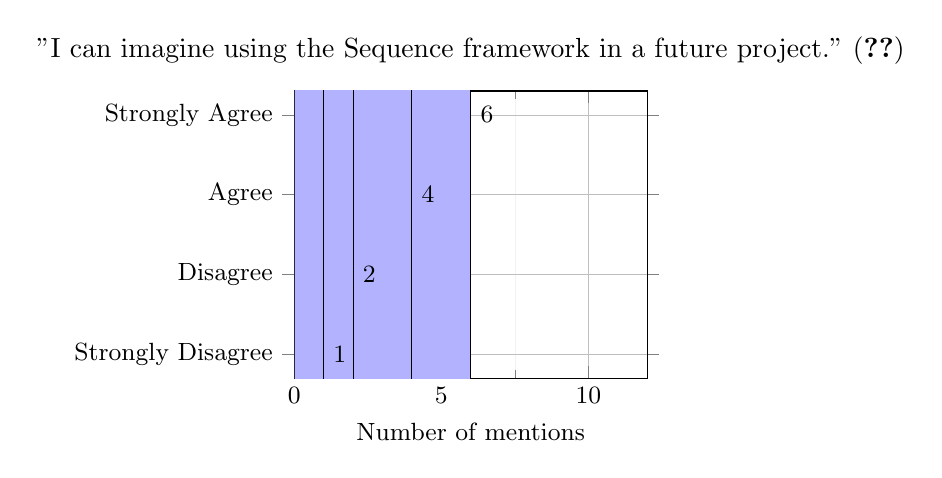
\begin{tikzpicture}
\begin{axis}[
% instead of scaling
width=\textwidth / 2, % Breite des Charts
title={"I can imagine using the Sequence framework in a future project."~(\ref{sub:ut_q4})},
xbar,  % Art des Charts                                            
xmin=0, % y min
xmax=12, % y max
%ylabel style={color=darkgray},
ticklabel style={font=\small},
label style={font=\small},
nodes near coords style={font=\small},
bar width=20, % Breite der Balken (in points)
nodes near coords, % Labels oberhalb der Bars
xlabel={Number of mentions},
grid=both, % Zeilen ds Grids
grid style={line width=.1pt, draw=gray!10},
major grid style={line width=.2pt,draw=gray!50},
minor x tick num=1,
ytick=data,
% use explicit ticklabels instead of symbolc x coords
yticklabels={Strongly Agree, Agree, Disagree, Strongly Disagree},
]
\addplot[black,fill=blue!30!white]
coordinates{ (6,4) (4,3) (2,2) (1,1) };
\end{axis}
\end{tikzpicture}
\caption{Responses to "I can imagine using the Sequence framework in a future project."}
\label{fig:usertest_q1}
\end{figure}
% subsubsection Conclusion (end)
% subsection Findings Sequence library(end)
\subsection{Findings for JINQ} % (fold)
\label{sub:Findings for JINQ}
\subsubsection{Findings and Improvements} % (fold)
\label{subsub:jinq_finding_and_imrpovements}

We decided to include following findings into JINQ:
\begin{itemize}
  \item \textbf{Better Introduction to JINQ}: Two people suggest using
    |JSONMonad()| directly inside of |from| (text answer~\ref{sub:ut_q13}).
    However, this makes no sense since JINQ can handle arbitrary monads. Thus,
    the documentation provided did not provide a sufficient overview.
    Therefore, the JSDoc of JINQ must give a better introduction to the topic.
    Additional examples should show the usage using different monads.
  \item \textbf{Revise JSDoc (functions and examples)}: Nearly a quarter of the participants found JINQ
    challenging (\ref{sub:ut_q8}). This shows that these concepts needed to be
    sufficiently well introduced. From the solutions given to us, it is evident
    that more JSDoc was required. In addition, more examples would coin to a
    better understanding (text answer~\ref{sub:ut_q13}).
    \item \textbf{Not exactly the same as SQL}: Two people needed help with
      JINQ not writing exactly like SQL (handed in code). An SQL query
      |Select NAME from PERSON where AGE > 18| is translated into JINQ via
      |from(PERSON).where(p => p.age > 18).select(p => p.name);| So the order
      of |select| and |where| is reversed. So the JSDoc of JINQ needs to
      mention more clearly that working with JINQ is different than working
      with SQL.
\end{itemize}

The following are great ideas but are beyond the scope of this project to
implement. Find detailed information about all of them in the
Section~\ref{sub:JINQ Functions}.
\begin{itemize}
  \item \textbf{Error handling}: Several people had trouble with null values,
    mainly when, for example, when calling a  function on a non-existent object
    property in a |select| or a |where| (text answer~\ref{sub:ut_q13}, and
    handed in solution). In the discussion, the idea came up to
    provide functions like |notNull|, |safeWhere| or |safeMap| to catch this.
\end{itemize}
% subsubsection Findings and Improvements (end)
\subsubsection{Conclusion} % (fold)
\label{subsub:Conclusion}
Although JINQ still has room for improvement, the general feedback is very
good. Almost all find it helpful to search JSON structures using JINQ
(\ref{sub:ut_q10}). The majority already found the current state of JINQ easy
to use \ref{sub:ut_q8}.

As Figure~\ref{fig:usertest_q2} shows, most people think that JINQ can be an asset in a future
project:
\begin{figure}[H]
\centering
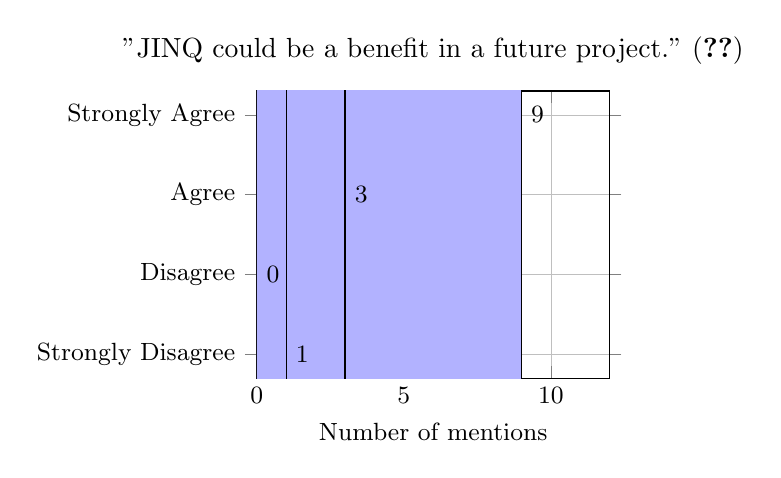
\begin{tikzpicture}
\begin{axis}[
% instead of scaling
width=\textwidth / 2, % Breite des Charts
title={"JINQ could be a benefit in a future project."~(\ref{sub:ut_q12})},
xbar,  % Art des Charts                                            
xmin=0, % y min
xmax=12, % y max
%ylabel style={color=darkgray},
ticklabel style={font=\small},
label style={font=\small},
nodes near coords style={font=\small},
bar width=20, % Breite der Balken (in points)
nodes near coords, % Labels oberhalb der Bars
xlabel={Number of mentions},
grid=both, % Zeilen ds Grids
grid style={line width=.1pt, draw=gray!10},
major grid style={line width=.2pt,draw=gray!50},
minor x tick num=1,
ytick=data,
% use explicit ticklabels instead of symbolc x coords
yticklabels={Strongly Agree, Agree, Disagree, Strongly Disagree},
]
\addplot[black,fill=blue!30!white]
coordinates{(9,4) (3,3) (0,2) (1,1)};
\end{axis}
\end{tikzpicture}
\caption{Responses to "JINQ could be a benefit in a future project."}
\label{fig:usertest_q2}
\end{figure}
% subsubsection Conclusion (end)
% subsection Findings for JINQ (end)
\subsection{General Findings} % (fold)
\label{sub:General Findings}
The questionnaire concludes with general questions. Among other things, the
closing explains how effectively IDEs support JSDoc and whether the testers
find this useful. Most participants used IntelliJ or WebStorm for testing
(~\ref{sub:ut_q15}). Figure~\ref{fig:usertest_q3} shows that the IDE was an excellent help for this test. Thus, It
makes sense to write a detailed JSDoc. Code navigation, code completion, etc.,
are also popular with users in JavaScript. With the right IDEs, this also works
very well.
%\begin{figure}[H]
%\begin{tikzpicture}
%\begin{axis}[
%% instead of scaling
%width=\textwidth / 2, % Breite des Charts
%title={"My IDE provided me with helpful support during the user test." (\ref{sub:ut_q16})},
%ybar,  % Art des Charts                                            
%ymin=0, % y min
%ymax=12, % y max
%%ylabel style={color=darkgray},
%%xlabel style={font=\small},
%bar width=20, % Breite der Balken (in points)
%nodes near coords, % Labels oberhalb der Bars
%ylabel={Number of mentions},
%grid=both, % Zeilen ds Grids
%grid style={line width=.1pt, draw=gray!10},
%major grid style={line width=.2pt,draw=gray!50},
%minor y tick num=4,
%xtick=data,
%% use explicit ticklabels instead of symbolc x coords
%xticklabels={Strongly Agree, Agree, Disagree, Strongly Disagree},
%xticklabel style={ rotate=-20 },
%]
%\addplot[black,fill=blue!30!white]
%coordinates{ (1,10) (2,2) (3,1) (4,0) };
%\end{axis}
%\end{tikzpicture}

\begin{figure}[H]
\centering
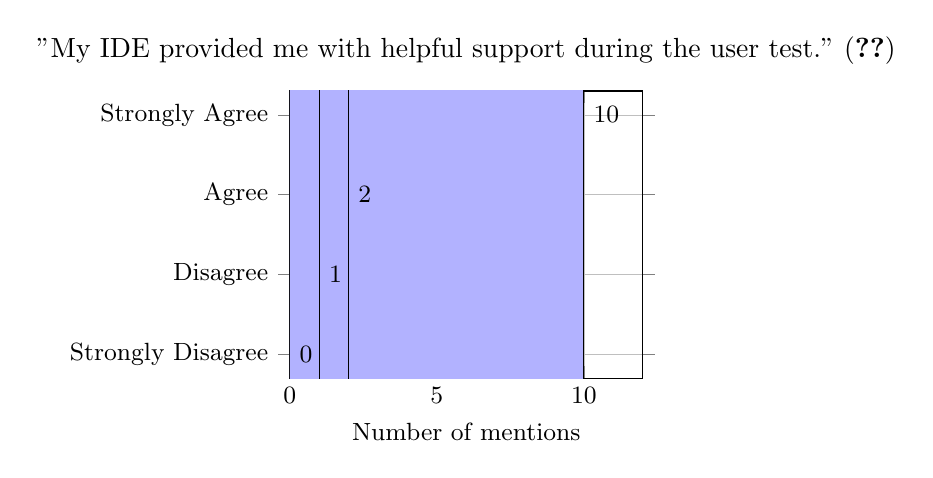
\begin{tikzpicture}
\begin{axis}[
% instead of scaling
width=\textwidth / 2, % Breite des Charts
title={"My IDE provided me with helpful support during the user test." (\ref{sub:ut_q16})},
xbar,  % Art des Charts                                            
xmin=0, % y min
xmax=12, % y max
%ylabel style={color=darkgray},
ticklabel style={font=\small},
label style={font=\small},
nodes near coords style={font=\small},
bar width=20, % Breite der Balken (in points)
nodes near coords, % Labels oberhalb der Bars
xlabel={Number of mentions},
grid=both, % Zeilen ds Grids
grid style={line width=.1pt, draw=gray!10},
major grid style={line width=.2pt,draw=gray!50},
minor x tick num=1,
ytick=data,
% use explicit ticklabels instead of symbolc x coords
yticklabels={Strongly Agree, Agree, Disagree, Strongly Disagree},
]
\addplot[black,fill=blue!30!white]
coordinates{ (10,4) (2,3) (1,2) (0,1) };
\end{axis}
\end{tikzpicture}
\caption{Responses to "My IDE provided me with helpful support during the user
test."}
\label{fig:usertest_q3}
\end{figure}

% subsection General Findings (end)
\subsection{Conclusion} % (fold)
\label{sub:Conclusion}

This user test shows that the features this library brings are beneficial. In
addition, it offers some improvement points of the API. Implementing the
documented hints improves the quality and usability of this library even more.
We are delighted with the result. Of course, we are especially pleased with the
text responses - many further underline the positive attitude towards this
library. 

% subsection Conclusion (end)
% section User Test Evaluation (end)
